%%%%%%%%%%%%%%%%%%%%%%%%%%%%%%%%%%%%%%%%%%%%%%%%%%%%%%%%%%%%%%%%%%%%%%%%%%%%%%%

\chapter{PROPOSTA}\label{ch:prop}

{\color{cerulean}
Esta seção apresenta os objetivos do trabalho, bem como a problemática dos dados disponíveis atualmente e apresenta a estrutura que é proposta para solucionar o problema.
}

\section{Objetivos}\label{ch:prop:obj}

{\color{red}

O objetivo principal deste trabalho é estabelecer o uso de cubo de dados para que o processamento de consultas OLAP, da área espacial, sejam executadas de forma eficiente considerando-se a alta dimensionalidade, elevado número de tuplas e alta cardinalidade dos dados.
Como objetivos secundários, este trabalho visa:

\begin{enumerate}
\item Identificar quais são as consultas relevantes para os operadores de satélite, e quais são as atividades de análise que podem ser expressas como consultas;
\item Criar uma representação dimensional do cubo de dados apropriada para as consultas identificadas, mapeando as medidas que são necessárias e quais os seus tipos;
\item Implementar a representação com as medidas em algoritmos da literatura e coletar os resultados da execução das consultas relevantes para os operadores;
\item Avaliar os resultados da implementação dos algoritmos e mostrar qual das abordagens é mais apropriada para o cenário da operação.
\end{enumerate}

}

\section{Algoritmos de construção do cubo}\label{ch:prop:cube}

{\color{cerulean}
Para esta proposta, vamos nos concentrar apenas na proposição de um algoritmo de computação do cubo de dados.
Uma das necessidades de usar algoritmos diferentes de cubo de dados está no número de dimensões que um certo cubo consegue realizar pesquisas: consultas com mais que 15 dimensões não são comummente(ou praticamente) executadas em alguns algoritmos, como o trabalho de~\citeonline{silva:2015:abordagensParaCubo} demonstra.

Como estabelecido na seção~\ref{ch:prop:data}, os dados de telemetria de interesse possuem muito mais do que o limite de comum de consultas em até 60 dimensões: com mais de 130 telemetrias para os satélites da família da SCD, e milhares para satélites maiores como o CBERS e o Amazônia, a execução de consultas complexas seria normalmente inviável nos algortimos de construção do cubo tradicionais.

A figura~\ref{fig:qualistructure} mostra uma visão geral da estrutura proposta.
Seguindo a revisão feita an seção~\ref{ch:corr:cube}, o uso do \textit{FragCubing} seria adotado dadas as características altamente dimensionais dos dados.
Porém, para essa proposta, seria adicionado classificador intermediário: esse classificador gera os relacionamentos interessantes, que seriam dados de entrada de um algortimo do \textit{FragCubing} modificado, que decidirá como o cubo de dados resultante será construído.

\begin{figure}[!htb]
	\caption{Estrutura proposta}\label{fig:qualistructure}
	\vspace{2mm}
	\begin{center}
		\resizebox{14cm}{!}{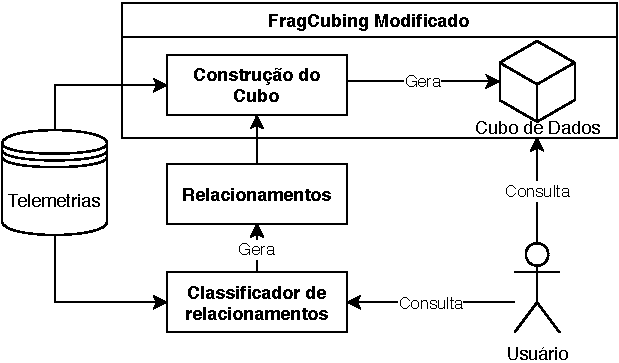
\includegraphics{Figuras/QualificationStructure.pdf}}
	\end{center}
	\vspace{1mm}
	\legenda{}
	\FONTE{Produção do autor.}
\end{figure}

Nessa estrutura, o usuário realiza consultas diretamente com o \textit{FragCubing} Modificado, porém como o classificador é uma ferramenta separada, ele pode ser utilizado de forma independente.
É importante ressaltar que o \textit{FragCubing} é composto de um algoritmo de construção do cubo e um algoritmo de processamento das consultas.

}
